\documentclass[tikz,dvipdfmx,dvipsnames]{standalone}

\usepackage{amsmath, amssymb, amsthm, mathrsfs, amsfonts, dsfont}
\usepackage{bbm}
\usepackage{bm}
\usepackage{physics}
\usepackage{ifthen}
\usepackage{setspace}
\usepackage{mathtools}

\newcommand{\defeq}{\coloneqq}

\newcommand{\red}[1]{\textcolor{red}{#1}}
\newcommand{\blue}[1]{\textcolor{blue}{#1}}
\newcommand{\cyan}[1]{\textcolor{cyan}{#1}}
\newcommand{\gray}[1]{\textcolor{gray}{#1}}
\newcommand{\green}[1]{\textcolor{green}{#1}}
\newcommand{\brown}[1]{\textcolor{brown}{#1}}
\newcommand{\black}[1]{\textcolor{black}{#1}}
\newcommand{\orange}[1]{\textcolor{orange}{#1}}
\newcommand{\purple}[1]{\textcolor{purple}{#1}}
\newcommand{\yellow}[1]{\textcolor{yellow}{#1}}
\newcommand{\Magenta}[1]{\textcolor{Magenta}{#1}}
\newcommand{\RoyalBlue}[1]{\textcolor{RoyalBlue}{#1}}
\newcommand{\RubineRed}[1]{\textcolor{RubineRed}{#1}}
\newcommand{\ForestGreen}[1]{\textcolor{ForestGreen}{#1}}
\newcommand{\YellowOrange}[1]{\textcolor{YellowOrange}{#1}}
\newcommand{\WildStrawberry}[1]{\textcolor{WildStrawberry}{#1}}

\usetikzlibrary{calc,matrix,math}
\usetikzlibrary{decorations.pathreplacing,calligraphy}

\definecolor{c0}{HTML}{64FF10}
\definecolor{c1}{HTML}{FF5785}

\begin{document}

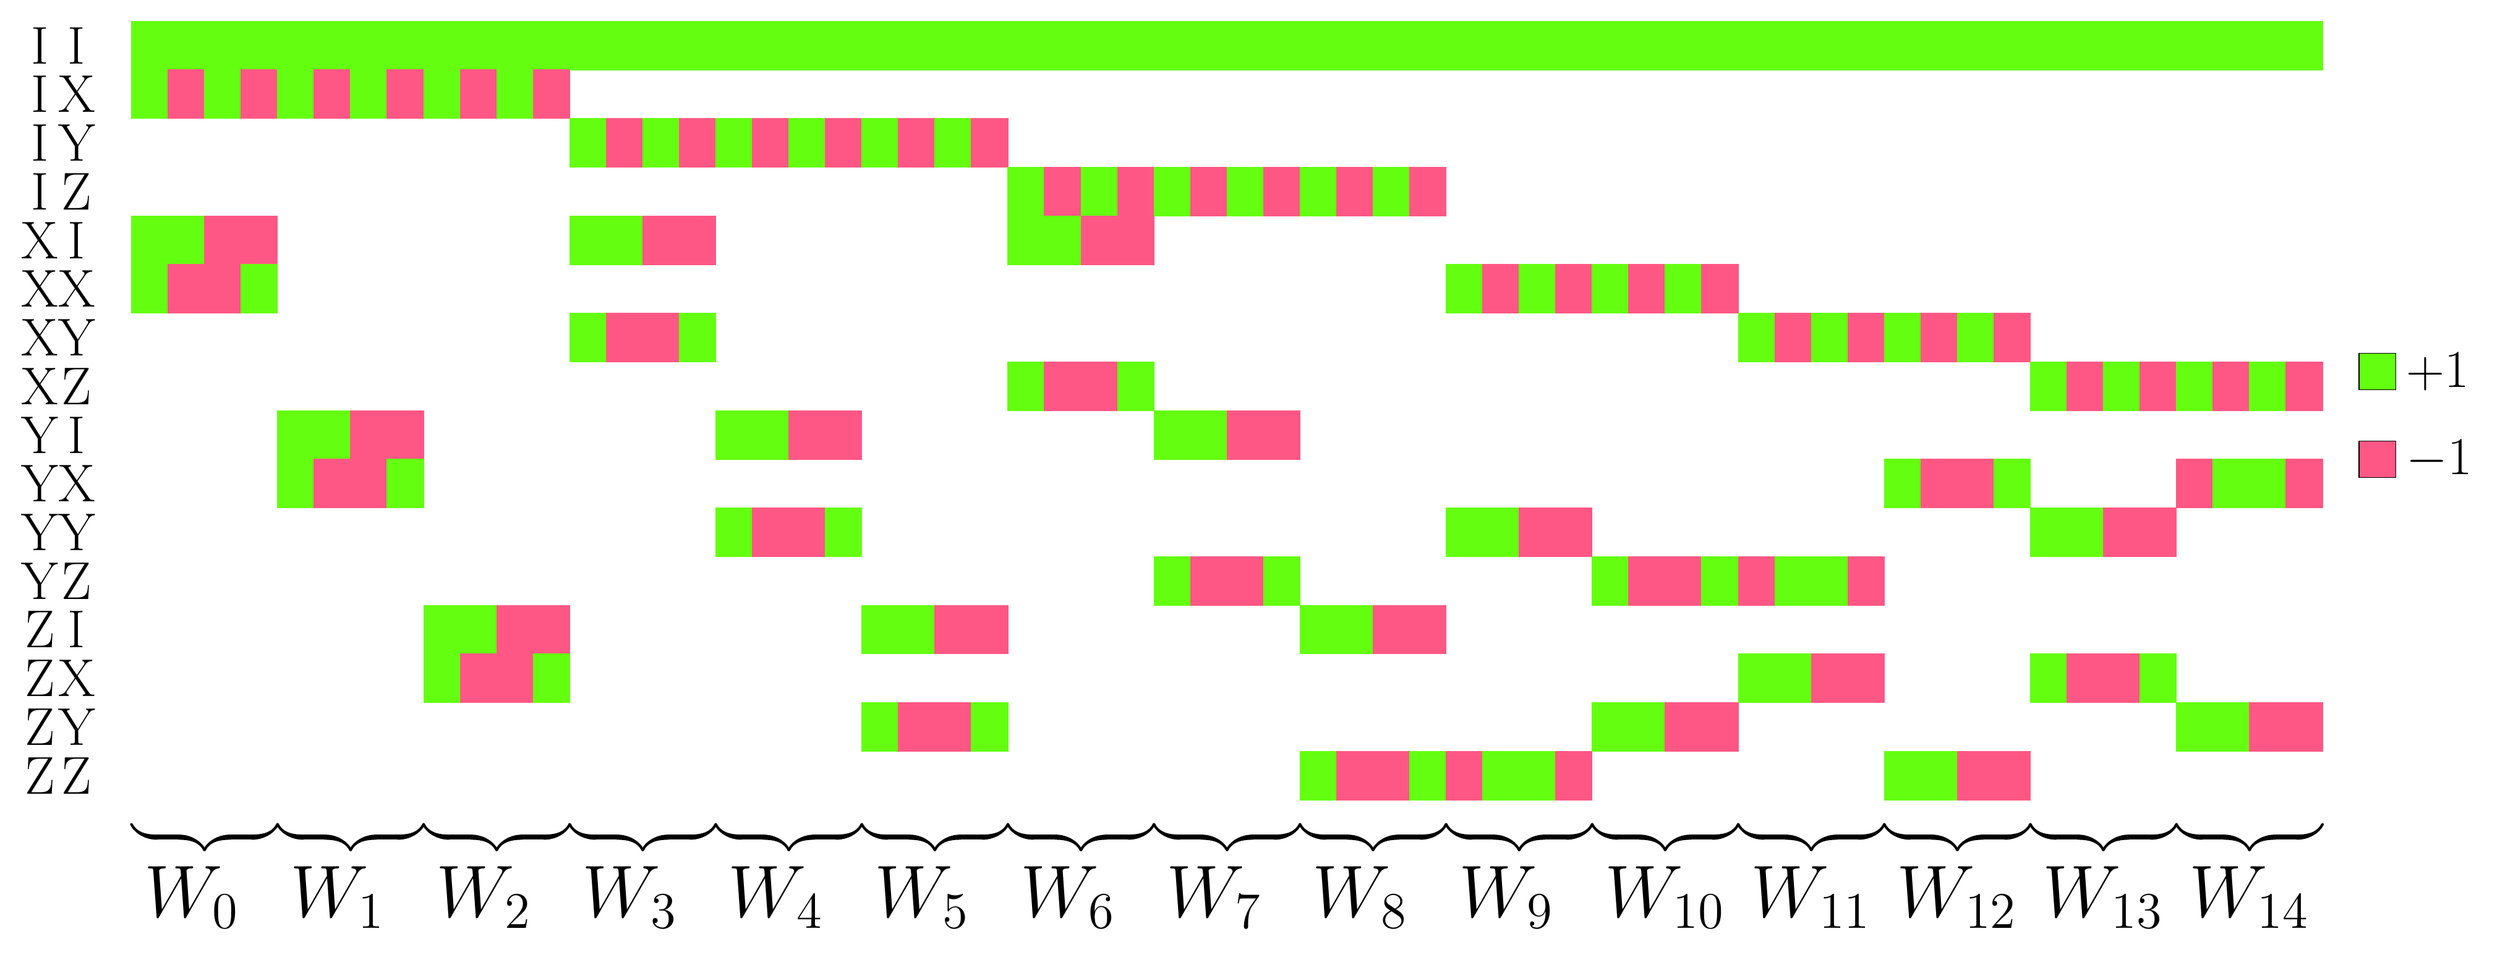
\begin{tikzpicture}[xscale=0.75]
    \foreach \color/\col/\row in {
            c0/0/0,
            c0/0/-1,
            c0/0/-4,
            c0/0/-5,
            c0/1/0,
            c1/1/-1,
            c0/1/-4,
            c1/1/-5,
            c0/2/0,
            c0/2/-1,
            c1/2/-4,
            c1/2/-5,
            c0/3/0,
            c1/3/-1,
            c1/3/-4,
            c0/3/-5,
            c0/4/0,
            c0/4/-1,
            c0/4/-8,
            c0/4/-9,
            c0/5/0,
            c1/5/-1,
            c0/5/-8,
            c1/5/-9,
            c0/6/0,
            c0/6/-1,
            c1/6/-8,
            c1/6/-9,
            c0/7/0,
            c1/7/-1,
            c1/7/-8,
            c0/7/-9,
            c0/8/0,
            c0/8/-1,
            c0/8/-12,
            c0/8/-13,
            c0/9/0,
            c1/9/-1,
            c0/9/-12,
            c1/9/-13,
            c0/10/0,
            c0/10/-1,
            c1/10/-12,
            c1/10/-13,
            c0/11/0,
            c1/11/-1,
            c1/11/-12,
            c0/11/-13,
            c0/12/0,
            c0/12/-2,
            c0/12/-4,
            c0/12/-6,
            c0/13/0,
            c1/13/-2,
            c0/13/-4,
            c1/13/-6,
            c0/14/0,
            c0/14/-2,
            c1/14/-4,
            c1/14/-6,
            c0/15/0,
            c1/15/-2,
            c1/15/-4,
            c0/15/-6,
            c0/16/0,
            c0/16/-2,
            c0/16/-8,
            c0/16/-10,
            c0/17/0,
            c1/17/-2,
            c0/17/-8,
            c1/17/-10,
            c0/18/0,
            c0/18/-2,
            c1/18/-8,
            c1/18/-10,
            c0/19/0,
            c1/19/-2,
            c1/19/-8,
            c0/19/-10,
            c0/20/0,
            c0/20/-2,
            c0/20/-12,
            c0/20/-14,
            c0/21/0,
            c1/21/-2,
            c0/21/-12,
            c1/21/-14,
            c0/22/0,
            c0/22/-2,
            c1/22/-12,
            c1/22/-14,
            c0/23/0,
            c1/23/-2,
            c1/23/-12,
            c0/23/-14,
            c0/24/0,
            c0/24/-3,
            c0/24/-4,
            c0/24/-7,
            c0/25/0,
            c1/25/-3,
            c0/25/-4,
            c1/25/-7,
            c0/26/0,
            c0/26/-3,
            c1/26/-4,
            c1/26/-7,
            c0/27/0,
            c1/27/-3,
            c1/27/-4,
            c0/27/-7,
            c0/28/0,
            c0/28/-3,
            c0/28/-8,
            c0/28/-11,
            c0/29/0,
            c1/29/-3,
            c0/29/-8,
            c1/29/-11,
            c0/30/0,
            c0/30/-3,
            c1/30/-8,
            c1/30/-11,
            c0/31/0,
            c1/31/-3,
            c1/31/-8,
            c0/31/-11,
            c0/32/0,
            c0/32/-3,
            c0/32/-12,
            c0/32/-15,
            c0/33/0,
            c1/33/-3,
            c0/33/-12,
            c1/33/-15,
            c0/34/0,
            c0/34/-3,
            c1/34/-12,
            c1/34/-15,
            c0/35/0,
            c1/35/-3,
            c1/35/-12,
            c0/35/-15,
            c0/36/0,
            c0/36/-5,
            c0/36/-10,
            c1/36/-15,
            c0/37/0,
            c1/37/-5,
            c0/37/-10,
            c0/37/-15,
            c0/38/0,
            c0/38/-5,
            c1/38/-10,
            c0/38/-15,
            c0/39/0,
            c1/39/-5,
            c1/39/-10,
            c1/39/-15,
            c0/40/0,
            c0/40/-5,
            c0/40/-14,
            c0/40/-11,
            c0/41/0,
            c1/41/-5,
            c0/41/-14,
            c1/41/-11,
            c0/42/0,
            c0/42/-5,
            c1/42/-14,
            c1/42/-11,
            c0/43/0,
            c1/43/-5,
            c1/43/-14,
            c0/43/-11,
            c0/44/0,
            c0/44/-6,
            c0/44/-13,
            c1/44/-11,
            c0/45/0,
            c1/45/-6,
            c0/45/-13,
            c0/45/-11,
            c0/46/0,
            c0/46/-6,
            c1/46/-13,
            c0/46/-11,
            c0/47/0,
            c1/47/-6,
            c1/47/-13,
            c1/47/-11,
            c0/48/0,
            c0/48/-6,
            c0/48/-15,
            c0/48/-9,
            c0/49/0,
            c1/49/-6,
            c0/49/-15,
            c1/49/-9,
            c0/50/0,
            c0/50/-6,
            c1/50/-15,
            c1/50/-9,
            c0/51/0,
            c1/51/-6,
            c1/51/-15,
            c0/51/-9,
            c0/52/0,
            c0/52/-7,
            c0/52/-10,
            c0/52/-13,
            c0/53/0,
            c1/53/-7,
            c0/53/-10,
            c1/53/-13,
            c0/54/0,
            c0/54/-7,
            c1/54/-10,
            c1/54/-13,
            c0/55/0,
            c1/55/-7,
            c1/55/-10,
            c0/55/-13,
            c0/56/0,
            c0/56/-7,
            c0/56/-14,
            c1/56/-9,
            c0/57/0,
            c1/57/-7,
            c0/57/-14,
            c0/57/-9,
            c0/58/0,
            c0/58/-7,
            c1/58/-14,
            c0/58/-9,
            c0/59/0,
            c1/59/-7,
            c1/59/-14,
            c1/59/-9
        }{
            \draw[
                fill=\color,
                draw=\color
            ] (\col, \row) rectangle (\col + 1, \row - 1);
        }

    \foreach \row/\label in {
            -0.5/ \makebox[0cm][c]{I}\phantom{X}\makebox[0cm][c]{I}\phantom{X},
            -1.5/ \makebox[0cm][c]{I}\phantom{X}\makebox[0cm][c]{X}\phantom{X},
            -2.5/ \makebox[0cm][c]{I}\phantom{X}\makebox[0cm][c]{Y}\phantom{X},
            -3.5/ \makebox[0cm][c]{I}\phantom{X}\makebox[0cm][c]{Z}\phantom{X},
            -4.5/ \makebox[0cm][c]{X}\phantom{X}\makebox[0cm][c]{I}\phantom{X},
            -5.5/ \makebox[0cm][c]{X}\phantom{X}\makebox[0cm][c]{X}\phantom{X},
            -6.5/ \makebox[0cm][c]{X}\phantom{X}\makebox[0cm][c]{Y}\phantom{X},
            -7.5/ \makebox[0cm][c]{X}\phantom{X}\makebox[0cm][c]{Z}\phantom{X},
            -8.5/ \makebox[0cm][c]{Y}\phantom{X}\makebox[0cm][c]{I}\phantom{X},
            -9.5/ \makebox[0cm][c]{Y}\phantom{X}\makebox[0cm][c]{X}\phantom{X},
            -10.5/\makebox[0cm][c]{Y}\phantom{X}\makebox[0cm][c]{Y}\phantom{X},
            -11.5/\makebox[0cm][c]{Y}\phantom{X}\makebox[0cm][c]{Z}\phantom{X},
            -12.5/\makebox[0cm][c]{Z}\phantom{X}\makebox[0cm][c]{I}\phantom{X},
            -13.5/\makebox[0cm][c]{Z}\phantom{X}\makebox[0cm][c]{X}\phantom{X},
            -14.5/\makebox[0cm][c]{Z}\phantom{X}\makebox[0cm][c]{Y}\phantom{X},
            -15.5/\makebox[0cm][c]{Z}\phantom{X}\makebox[0cm][c]{Z}\phantom{X}
        }{
            \node[anchor=center,font=\LARGE,scale=1.8]
            at (-1.5, \row) {\label};
        }

    \foreach \l/\r/\k in {
            0/4/0,
            4/8/1,
            8/12/2,
            12/16/3,
            16/20/4,
            20/24/5,
            24/28/6,
            28/32/7,
            32/36/8,
            36/40/9,
            40/44/10,
            44/48/11,
            48/52/12,
            52/56/13,
            56/60/14
        }{
            \draw[decorate,
                decoration={calligraphic brace,mirror,amplitude=15pt},
                line width=3pt]
            (\l, -16.5) -- (\r, -16.5)
            node[
                midway, yshift=-1.5cm, font=\LARGE, scale=2.5
            ] {$W_{\mathrlap{\k}\phantom{11}}$};
        }

    \begin{scope}[yscale=0.75,xshift=61cm]
        \draw[fill=c0] (0, -0.7-1.2*7) rectangle (1, -0.7-1.2*7-1);
        \draw[fill=c1] (0, -0.7-1.2*9) rectangle (1, -0.7-1.2*9-1);
        \node[anchor=west,font=\LARGE,scale=1.8] at (1, -0.7-1.2*7-0.5) {$+1$};
        \node[anchor=west,font=\LARGE,scale=1.8] at (1, -0.7-1.2*9-0.5) {$-1$};
    \end{scope}

    % margin
    \node at (-2.8, -17) {\phantom{X}};
\end{tikzpicture}

\end{document}